% =====================================================================
%  BUỔI 4 — TÀI LIỆU BUỔI HỌC (từ hoc-sinh/02-tai-lieu-buoi-hoc.md)
%  Sinh tự động bằng scripts/md2tex-chung.py — không sửa tay.
% =====================================================================
\documentclass[11pt, a4paper]{article}
% =====================================================================
%  CAE SHANGHAI — GÓI LỆNH DÙNG CHUNG CHO TÀI LIỆU LUYỆN THI CSCA TOÁN
%  Biên dịch bằng XeLaTeX. Mọi file .tex trong buổi học \input file này.
% =====================================================================

% ---------- NGÔN NGỮ & PHÔNG CHỮ ----------
\usepackage{fontspec}
\usepackage{polyglossia}
\setmainlanguage{vietnamese}
\setotherlanguage{english}

% Chữ Latin (Anh + Việt): TeX Gyre Termes — bản clone Times New Roman,
% đi kèm TeX Live, hỗ trợ đầy đủ dấu tiếng Việt.
\setmainfont{TeX Gyre Termes}
\setsansfont{TeX Gyre Heros}

% Chữ Hán: ưu tiên Source Han Serif SC (思源宋体) — chuẩn học thuật Trung Quốc.
% Nếu máy chưa cài, tự động dùng Songti SC (宋体, có sẵn trên macOS).
% Cả hai đều thuộc họ 宋体 nên diện mạo tài liệu không đổi.
\IfFontExistsTF{Source Han Serif SC}{
  \newcommand{\cjkfamilyname}{Source Han Serif SC}
}{
  \IfFontExistsTF{Songti SC}{
    \newcommand{\cjkfamilyname}{Songti SC}
  }{
    \newcommand{\cjkfamilyname}{Noto Serif CJK SC}
  }
}

% xeCJK tự chuyển font khi gặp ký tự Hán, không cần bọc \cjk{} thủ công.
% Đây là điều kiện bắt buộc: font Latin (TeX Gyre Termes) không có glyph chữ Hán,
% nếu không khai báo xeCJK thì mọi chữ Hán viết trần sẽ bị nuốt khỏi bản in.
\usepackage{xeCJK}
\setCJKfamilyfont{caehan}{\cjkfamilyname}[Scale=0.95]
\setCJKmainfont{\cjkfamilyname}[Scale=0.95]
\setCJKsansfont{\cjkfamilyname}[Scale=0.95]
\setCJKmonofont{\cjkfamilyname}[Scale=0.95]

% \cjk{} ép dùng font Hán trong ngữ cảnh cần thiết (ví dụ trong tiêu đề in đậm
% hoặc trong bảng có định dạng riêng). Dùng \CJKfamily chứ không phải tên font,
% vì tên font chỉ là văn bản — sẽ in ra chữ thay vì đổi font.
\newcommand{\cjk}[1]{{\CJKfamily{caehan}#1}}

% ---------- TOÁN HỌC ----------
\usepackage{amsmath, amssymb, amsthm, mathtools}
\usepackage{unicode-math}
\setmathfont{TeX Gyre Termes Math}

% ---------- BỐ CỤC TRANG ----------
% Lề phải chừa vùng an toàn của letterhead:
%   banner trên chiếm 0–19mm  → top tối thiểu 2,2cm
%   banner dưới chiếm 281–297mm → bottom tối thiểu 2,2cm
% Lề trên 2,6cm (26mm) để tiêu đề đầu trang không đè banner (banner hết ở 19mm).
\usepackage[a4paper, top=2.6cm, bottom=2.4cm, left=2.5cm, right=2.0cm]{geometry}
\usepackage{fancyhdr}
\usepackage{titlesec}
\usepackage{enumitem}
\usepackage{graphicx}
\usepackage{booktabs, array, longtable, tabularx}
\usepackage{xcolor}
\usepackage[most]{tcolorbox}
\usepackage[colorlinks=true, linkcolor=cae_blue, citecolor=cae_blue, urlcolor=cae_blue]{hyperref}

% ---------- BẢNG MÀU THƯƠNG HIỆU ----------
\definecolor{cae_blue}{RGB}{0, 51, 102}
\definecolor{cae_gold}{RGB}{196, 149, 60}
\definecolor{box_bg}{RGB}{245, 247, 250}
\definecolor{box_line}{RGB}{0, 51, 102}

% ---------- TIÊU ĐỀ MỤC ----------
% Đệm đầu trang: banner letterhead chiếm 0–19mm, mà lề trên là 22mm.
% \section* đầu trang (sau \clearpage) sát lề nên phải chừa thêm, nếu không
% sẽ đè lên banner.
\titleformat{\section}
  {\normalfont\large\bfseries\sffamily\color{cae_blue}}{\thesection.}{0.6em}{}
\titleformat{\subsection}
  {\normalfont\normalsize\bfseries\sffamily\color{cae_blue!85!black}}{\thesubsection}{0.6em}{}
\titlespacing*{\section}{0pt}{14pt}{6pt}
\titlespacing*{\subsection}{0pt}{10pt}{4pt}

% Tiêu đề không đánh số ở đầu trang: \section* sau \clearpage nằm sát lề trên
% nên đè lên banner letterhead. Dùng \vspace* ngay TRƯỚC \section* không đủ,
% vì titlesec chèn khoảng cách riêng. Cách chắc chắn là đệm bằng \null.
\newcommand{\sectiondautrang}[1]{\section*{#1}}

% Dạng bài dùng \subsection*{} nên cần định dạng riêng, đậm và có gạch chân màu
\titleformat{\subsubsection}
  {\normalfont\normalsize\bfseries\sffamily\color{cae_blue!85!black}}{\thesubsubsection}{0.6em}{}

% ---------- LETTERHEAD (ảnh nền toàn trang) ----------
% Ảnh letterhead của CAE Shanghai: banner xanh trên/dưới kèm logo chìm giữa.
% Tỉ lệ ảnh 1414x2000 = 0.7070, khớp A4 (0.7071) nên chèn thẳng không méo.
% Đặt ở lớp nền dưới cùng để chữ không bị ảnh che.
% Dùng \AddToShipoutPictureBG (không có dấu *) để áp dụng cho MỌI trang.
\usepackage{eso-pic}
\AddToShipoutPictureBG{%
  \AtPageLowerLeft{%
    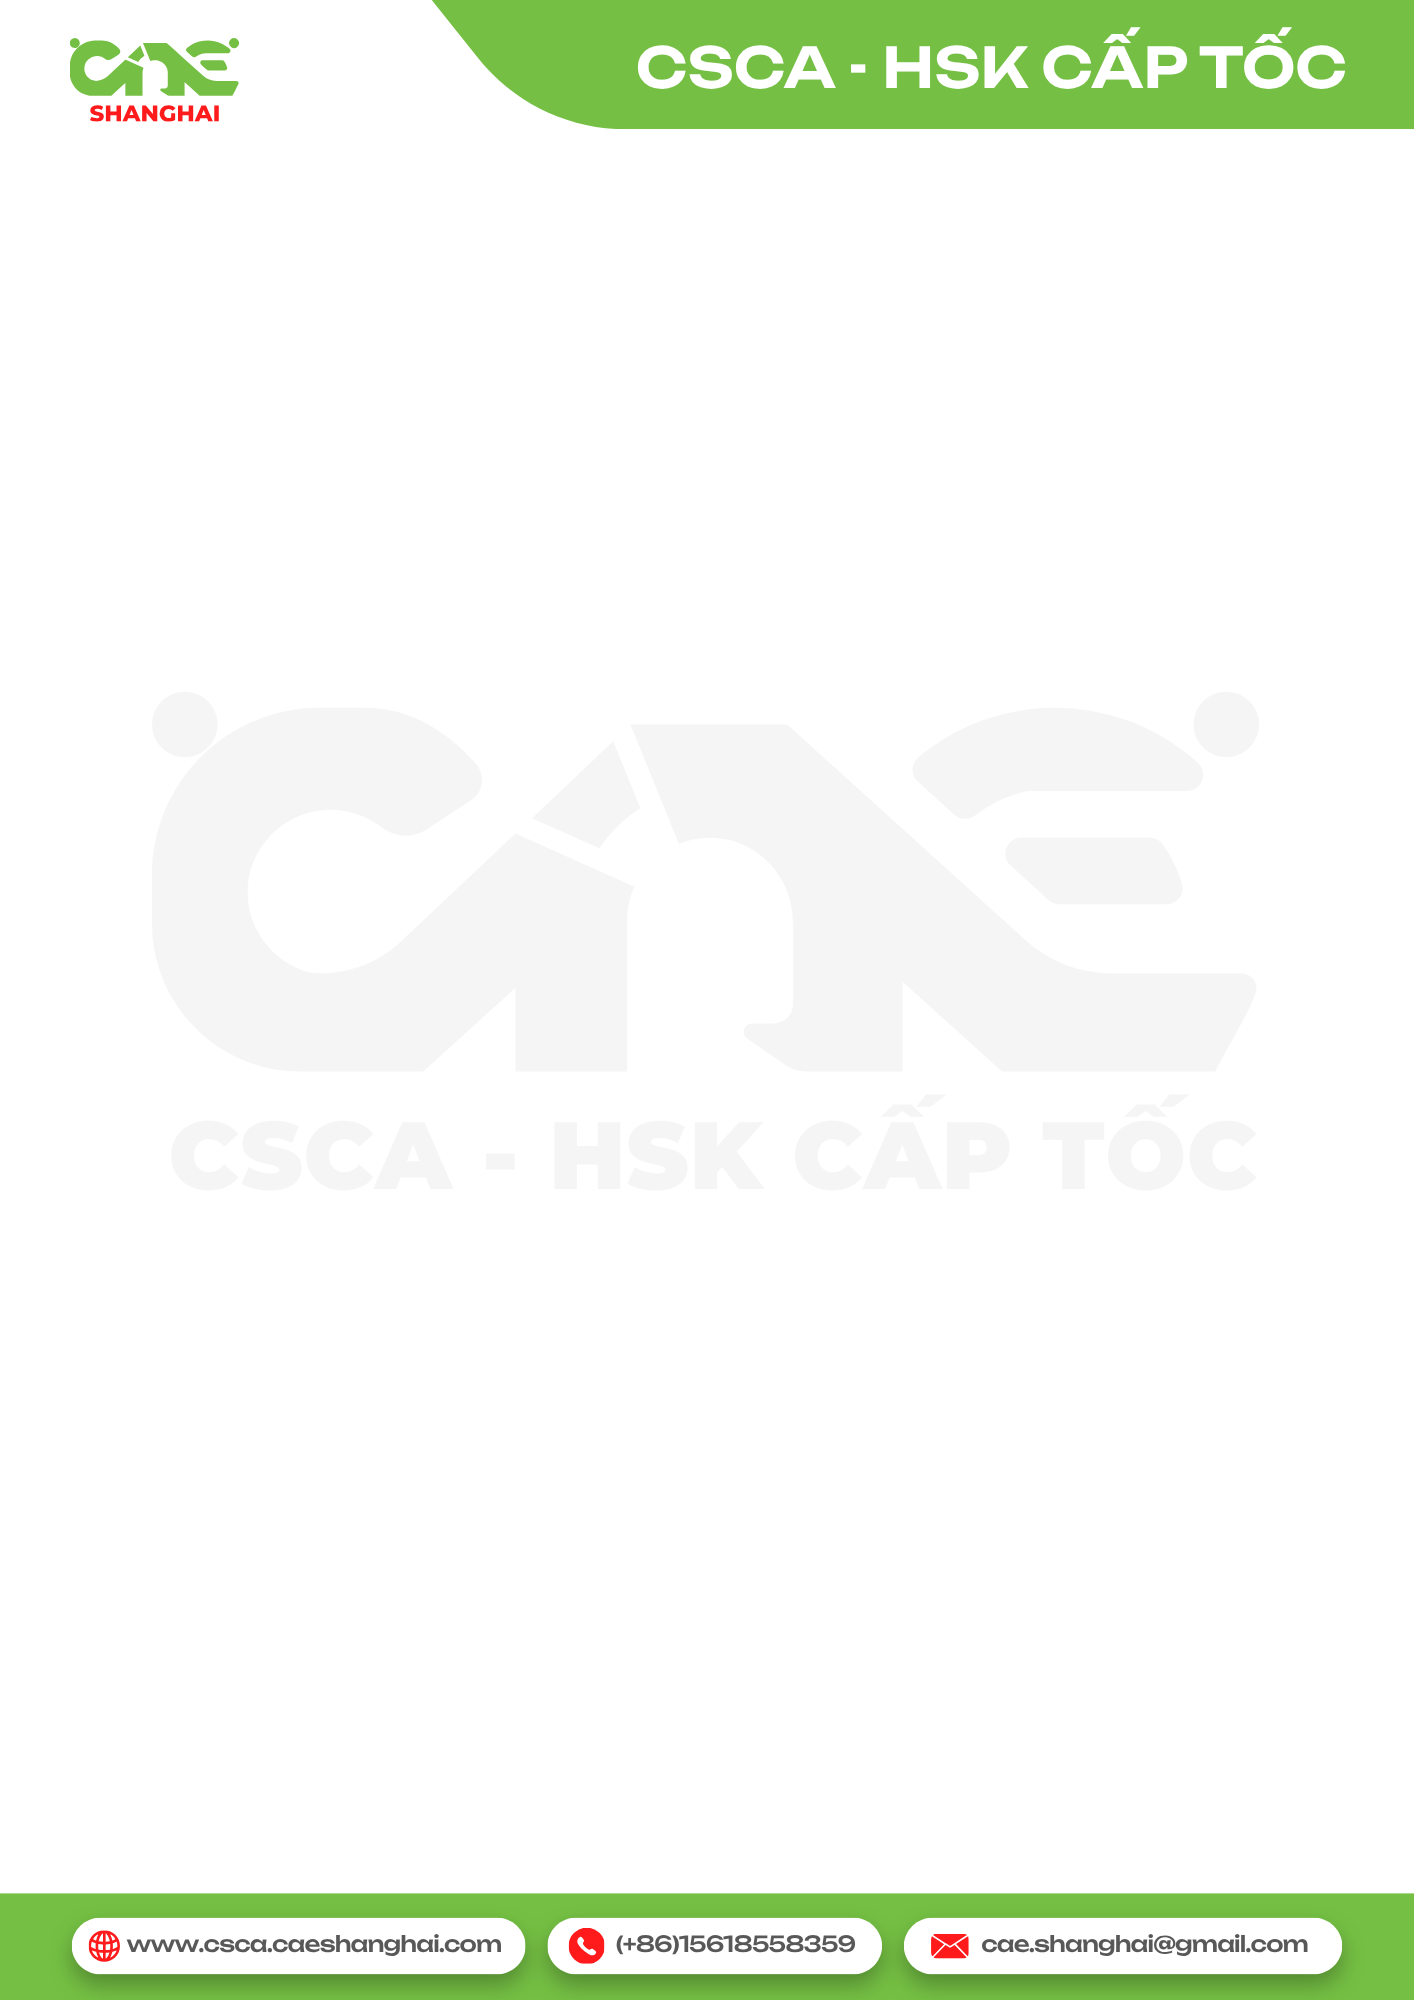
\includegraphics[width=\paperwidth,height=\paperheight]{images/letterhead.png}%
  }%
}

% ---------- ĐẦU / CHÂN TRANG ----------
% Letterhead đã có banner trên và dưới, nên bỏ dòng chạy để tránh chồng chữ.
% Số trang đặt trong vùng nội dung, sát trên banner dưới, lề phải.
\pagestyle{fancy}
\setlength{\headheight}{0pt}
\fancyhf{}
\renewcommand{\headrulewidth}{0pt}
\renewcommand{\footrulewidth}{0pt}
\fancyfoot[R]{\raisebox{0.9cm}{\small\color{cae_blue}\thepage}}

% ---------- MÔI TRƯỜNG NỘI DUNG ----------
% Trong tcolorbox, LaTeX đặt parindent = parskip = 0, nên các đoạn văn trong
% khung dính liền nhau. Đặt lại khoảng cách đoạn cho mọi khung.
\newcommand{\khoangcachdoan}{\setlength{\parskip}{0.5em}\setlength{\parindent}{0pt}}
\tcbset{before upper={\khoangcachdoan}}

\newtcolorbox{dinhnghia}[1][]{
  colback=box_bg, colframe=box_line, boxrule=0.6pt, arc=1pt,
  fonttitle=\bfseries, title={Định nghĩa #1}, breakable}
\newtcolorbox{dinhly}[1][]{
  colback=box_bg, colframe=cae_gold, boxrule=0.6pt, arc=1pt,
  fonttitle=\bfseries, title={Tính chất #1}, breakable}
\newtcolorbox{vidu}[1][]{
  colback=white, colframe=black!40, boxrule=0.4pt, arc=1pt,
  fonttitle=\bfseries, title={Ví dụ #1}, breakable}
\newtcolorbox{baitap}[1][]{
  colback=white, colframe=cae_blue!50, boxrule=0.4pt, arc=1pt,
  fonttitle=\bfseries, title={Câu #1}, breakable}

% Ô đáp án: viền xanh đậm hơn, dùng trong file đáp án
\newtcolorbox{dapan}[1][]{
  colback=box_bg, colframe=cae_blue, boxrule=0.6pt, arc=1pt,
  fonttitle=\bfseries, title={Câu #1}, breakable}

% ---------- TÊN CHỨNG MINH ----------
\renewcommand{\proofname}{\normalfont\bfseries Chứng minh}

% ---------- MÔN HỌC ----------
% Đổi được ở file .tex trước khi % =====================================================================
%  CAE SHANGHAI — GÓI LỆNH DÙNG CHUNG CHO TÀI LIỆU LUYỆN THI CSCA TOÁN
%  Biên dịch bằng XeLaTeX. Mọi file .tex trong buổi học \input file này.
% =====================================================================

% ---------- NGÔN NGỮ & PHÔNG CHỮ ----------
\usepackage{fontspec}
\usepackage{polyglossia}
\setmainlanguage{vietnamese}
\setotherlanguage{english}

% Chữ Latin (Anh + Việt): TeX Gyre Termes — bản clone Times New Roman,
% đi kèm TeX Live, hỗ trợ đầy đủ dấu tiếng Việt.
\setmainfont{TeX Gyre Termes}
\setsansfont{TeX Gyre Heros}

% Chữ Hán: ưu tiên Source Han Serif SC (思源宋体) — chuẩn học thuật Trung Quốc.
% Nếu máy chưa cài, tự động dùng Songti SC (宋体, có sẵn trên macOS).
% Cả hai đều thuộc họ 宋体 nên diện mạo tài liệu không đổi.
\IfFontExistsTF{Source Han Serif SC}{
  \newcommand{\cjkfamilyname}{Source Han Serif SC}
}{
  \IfFontExistsTF{Songti SC}{
    \newcommand{\cjkfamilyname}{Songti SC}
  }{
    \newcommand{\cjkfamilyname}{Noto Serif CJK SC}
  }
}

% xeCJK tự chuyển font khi gặp ký tự Hán, không cần bọc \cjk{} thủ công.
% Đây là điều kiện bắt buộc: font Latin (TeX Gyre Termes) không có glyph chữ Hán,
% nếu không khai báo xeCJK thì mọi chữ Hán viết trần sẽ bị nuốt khỏi bản in.
\usepackage{xeCJK}
\setCJKfamilyfont{caehan}{\cjkfamilyname}[Scale=0.95]
\setCJKmainfont{\cjkfamilyname}[Scale=0.95]
\setCJKsansfont{\cjkfamilyname}[Scale=0.95]
\setCJKmonofont{\cjkfamilyname}[Scale=0.95]

% \cjk{} ép dùng font Hán trong ngữ cảnh cần thiết (ví dụ trong tiêu đề in đậm
% hoặc trong bảng có định dạng riêng). Dùng \CJKfamily chứ không phải tên font,
% vì tên font chỉ là văn bản — sẽ in ra chữ thay vì đổi font.
\newcommand{\cjk}[1]{{\CJKfamily{caehan}#1}}

% ---------- TOÁN HỌC ----------
\usepackage{amsmath, amssymb, amsthm, mathtools}
\usepackage{unicode-math}
\setmathfont{TeX Gyre Termes Math}

% ---------- BỐ CỤC TRANG ----------
% Lề phải chừa vùng an toàn của letterhead:
%   banner trên chiếm 0–19mm  → top tối thiểu 2,2cm
%   banner dưới chiếm 281–297mm → bottom tối thiểu 2,2cm
% Lề trên 2,6cm (26mm) để tiêu đề đầu trang không đè banner (banner hết ở 19mm).
\usepackage[a4paper, top=2.6cm, bottom=2.4cm, left=2.5cm, right=2.0cm]{geometry}
\usepackage{fancyhdr}
\usepackage{titlesec}
\usepackage{enumitem}
\usepackage{graphicx}
\usepackage{booktabs, array, longtable, tabularx}
\usepackage{xcolor}
\usepackage[most]{tcolorbox}
\usepackage[colorlinks=true, linkcolor=cae_blue, citecolor=cae_blue, urlcolor=cae_blue]{hyperref}

% ---------- BẢNG MÀU THƯƠNG HIỆU ----------
\definecolor{cae_blue}{RGB}{0, 51, 102}
\definecolor{cae_gold}{RGB}{196, 149, 60}
\definecolor{box_bg}{RGB}{245, 247, 250}
\definecolor{box_line}{RGB}{0, 51, 102}

% ---------- TIÊU ĐỀ MỤC ----------
% Đệm đầu trang: banner letterhead chiếm 0–19mm, mà lề trên là 22mm.
% \section* đầu trang (sau \clearpage) sát lề nên phải chừa thêm, nếu không
% sẽ đè lên banner.
\titleformat{\section}
  {\normalfont\large\bfseries\sffamily\color{cae_blue}}{\thesection.}{0.6em}{}
\titleformat{\subsection}
  {\normalfont\normalsize\bfseries\sffamily\color{cae_blue!85!black}}{\thesubsection}{0.6em}{}
\titlespacing*{\section}{0pt}{14pt}{6pt}
\titlespacing*{\subsection}{0pt}{10pt}{4pt}

% Tiêu đề không đánh số ở đầu trang: \section* sau \clearpage nằm sát lề trên
% nên đè lên banner letterhead. Dùng \vspace* ngay TRƯỚC \section* không đủ,
% vì titlesec chèn khoảng cách riêng. Cách chắc chắn là đệm bằng \null.
\newcommand{\sectiondautrang}[1]{\section*{#1}}

% Dạng bài dùng \subsection*{} nên cần định dạng riêng, đậm và có gạch chân màu
\titleformat{\subsubsection}
  {\normalfont\normalsize\bfseries\sffamily\color{cae_blue!85!black}}{\thesubsubsection}{0.6em}{}

% ---------- LETTERHEAD (ảnh nền toàn trang) ----------
% Ảnh letterhead của CAE Shanghai: banner xanh trên/dưới kèm logo chìm giữa.
% Tỉ lệ ảnh 1414x2000 = 0.7070, khớp A4 (0.7071) nên chèn thẳng không méo.
% Đặt ở lớp nền dưới cùng để chữ không bị ảnh che.
% Dùng \AddToShipoutPictureBG (không có dấu *) để áp dụng cho MỌI trang.
\usepackage{eso-pic}
\AddToShipoutPictureBG{%
  \AtPageLowerLeft{%
    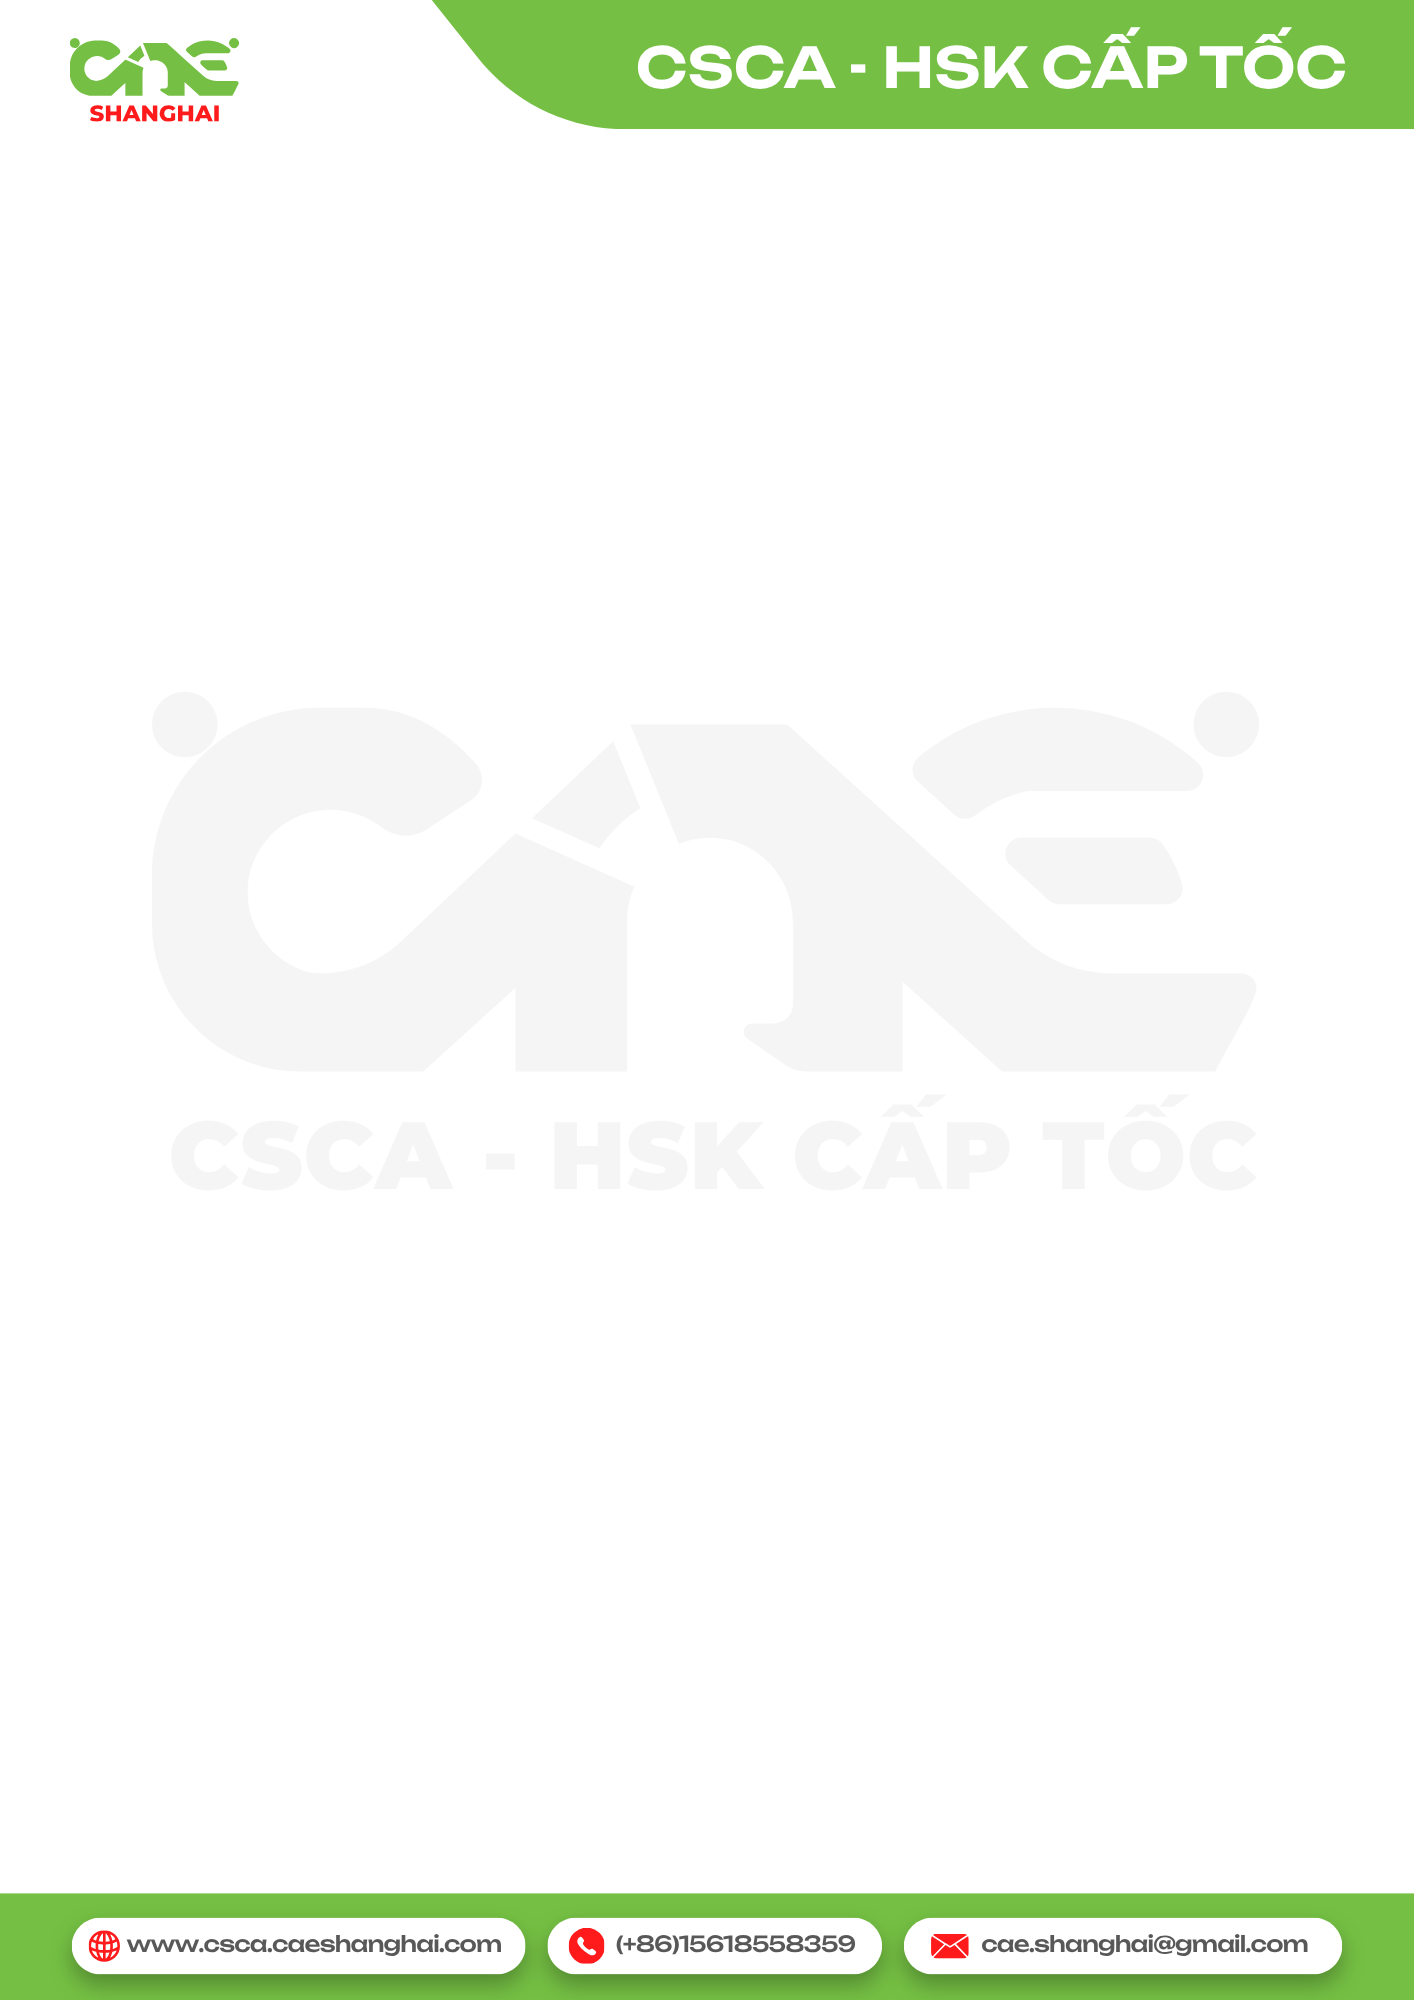
\includegraphics[width=\paperwidth,height=\paperheight]{images/letterhead.png}%
  }%
}

% ---------- ĐẦU / CHÂN TRANG ----------
% Letterhead đã có banner trên và dưới, nên bỏ dòng chạy để tránh chồng chữ.
% Số trang đặt trong vùng nội dung, sát trên banner dưới, lề phải.
\pagestyle{fancy}
\setlength{\headheight}{0pt}
\fancyhf{}
\renewcommand{\headrulewidth}{0pt}
\renewcommand{\footrulewidth}{0pt}
\fancyfoot[R]{\raisebox{0.9cm}{\small\color{cae_blue}\thepage}}

% ---------- MÔI TRƯỜNG NỘI DUNG ----------
% Trong tcolorbox, LaTeX đặt parindent = parskip = 0, nên các đoạn văn trong
% khung dính liền nhau. Đặt lại khoảng cách đoạn cho mọi khung.
\newcommand{\khoangcachdoan}{\setlength{\parskip}{0.5em}\setlength{\parindent}{0pt}}
\tcbset{before upper={\khoangcachdoan}}

\newtcolorbox{dinhnghia}[1][]{
  colback=box_bg, colframe=box_line, boxrule=0.6pt, arc=1pt,
  fonttitle=\bfseries, title={Định nghĩa #1}, breakable}
\newtcolorbox{dinhly}[1][]{
  colback=box_bg, colframe=cae_gold, boxrule=0.6pt, arc=1pt,
  fonttitle=\bfseries, title={Tính chất #1}, breakable}
\newtcolorbox{vidu}[1][]{
  colback=white, colframe=black!40, boxrule=0.4pt, arc=1pt,
  fonttitle=\bfseries, title={Ví dụ #1}, breakable}
\newtcolorbox{baitap}[1][]{
  colback=white, colframe=cae_blue!50, boxrule=0.4pt, arc=1pt,
  fonttitle=\bfseries, title={Câu #1}, breakable}

% Ô đáp án: viền xanh đậm hơn, dùng trong file đáp án
\newtcolorbox{dapan}[1][]{
  colback=box_bg, colframe=cae_blue, boxrule=0.6pt, arc=1pt,
  fonttitle=\bfseries, title={Câu #1}, breakable}

% ---------- TÊN CHỨNG MINH ----------
\renewcommand{\proofname}{\normalfont\bfseries Chứng minh}

% ---------- MÔN HỌC ----------
% Đổi được ở file .tex trước khi % =====================================================================
%  CAE SHANGHAI — GÓI LỆNH DÙNG CHUNG CHO TÀI LIỆU LUYỆN THI CSCA TOÁN
%  Biên dịch bằng XeLaTeX. Mọi file .tex trong buổi học \input file này.
% =====================================================================

% ---------- NGÔN NGỮ & PHÔNG CHỮ ----------
\usepackage{fontspec}
\usepackage{polyglossia}
\setmainlanguage{vietnamese}
\setotherlanguage{english}

% Chữ Latin (Anh + Việt): TeX Gyre Termes — bản clone Times New Roman,
% đi kèm TeX Live, hỗ trợ đầy đủ dấu tiếng Việt.
\setmainfont{TeX Gyre Termes}
\setsansfont{TeX Gyre Heros}

% Chữ Hán: ưu tiên Source Han Serif SC (思源宋体) — chuẩn học thuật Trung Quốc.
% Nếu máy chưa cài, tự động dùng Songti SC (宋体, có sẵn trên macOS).
% Cả hai đều thuộc họ 宋体 nên diện mạo tài liệu không đổi.
\IfFontExistsTF{Source Han Serif SC}{
  \newcommand{\cjkfamilyname}{Source Han Serif SC}
}{
  \IfFontExistsTF{Songti SC}{
    \newcommand{\cjkfamilyname}{Songti SC}
  }{
    \newcommand{\cjkfamilyname}{Noto Serif CJK SC}
  }
}

% xeCJK tự chuyển font khi gặp ký tự Hán, không cần bọc \cjk{} thủ công.
% Đây là điều kiện bắt buộc: font Latin (TeX Gyre Termes) không có glyph chữ Hán,
% nếu không khai báo xeCJK thì mọi chữ Hán viết trần sẽ bị nuốt khỏi bản in.
\usepackage{xeCJK}
\setCJKfamilyfont{caehan}{\cjkfamilyname}[Scale=0.95]
\setCJKmainfont{\cjkfamilyname}[Scale=0.95]
\setCJKsansfont{\cjkfamilyname}[Scale=0.95]
\setCJKmonofont{\cjkfamilyname}[Scale=0.95]

% \cjk{} ép dùng font Hán trong ngữ cảnh cần thiết (ví dụ trong tiêu đề in đậm
% hoặc trong bảng có định dạng riêng). Dùng \CJKfamily chứ không phải tên font,
% vì tên font chỉ là văn bản — sẽ in ra chữ thay vì đổi font.
\newcommand{\cjk}[1]{{\CJKfamily{caehan}#1}}

% ---------- TOÁN HỌC ----------
\usepackage{amsmath, amssymb, amsthm, mathtools}
\usepackage{unicode-math}
\setmathfont{TeX Gyre Termes Math}

% ---------- BỐ CỤC TRANG ----------
% Lề phải chừa vùng an toàn của letterhead:
%   banner trên chiếm 0–19mm  → top tối thiểu 2,2cm
%   banner dưới chiếm 281–297mm → bottom tối thiểu 2,2cm
% Lề trên 2,6cm (26mm) để tiêu đề đầu trang không đè banner (banner hết ở 19mm).
\usepackage[a4paper, top=2.6cm, bottom=2.4cm, left=2.5cm, right=2.0cm]{geometry}
\usepackage{fancyhdr}
\usepackage{titlesec}
\usepackage{enumitem}
\usepackage{graphicx}
\usepackage{booktabs, array, longtable, tabularx}
\usepackage{xcolor}
\usepackage[most]{tcolorbox}
\usepackage[colorlinks=true, linkcolor=cae_blue, citecolor=cae_blue, urlcolor=cae_blue]{hyperref}

% ---------- BẢNG MÀU THƯƠNG HIỆU ----------
\definecolor{cae_blue}{RGB}{0, 51, 102}
\definecolor{cae_gold}{RGB}{196, 149, 60}
\definecolor{box_bg}{RGB}{245, 247, 250}
\definecolor{box_line}{RGB}{0, 51, 102}

% ---------- TIÊU ĐỀ MỤC ----------
% Đệm đầu trang: banner letterhead chiếm 0–19mm, mà lề trên là 22mm.
% \section* đầu trang (sau \clearpage) sát lề nên phải chừa thêm, nếu không
% sẽ đè lên banner.
\titleformat{\section}
  {\normalfont\large\bfseries\sffamily\color{cae_blue}}{\thesection.}{0.6em}{}
\titleformat{\subsection}
  {\normalfont\normalsize\bfseries\sffamily\color{cae_blue!85!black}}{\thesubsection}{0.6em}{}
\titlespacing*{\section}{0pt}{14pt}{6pt}
\titlespacing*{\subsection}{0pt}{10pt}{4pt}

% Tiêu đề không đánh số ở đầu trang: \section* sau \clearpage nằm sát lề trên
% nên đè lên banner letterhead. Dùng \vspace* ngay TRƯỚC \section* không đủ,
% vì titlesec chèn khoảng cách riêng. Cách chắc chắn là đệm bằng \null.
\newcommand{\sectiondautrang}[1]{\section*{#1}}

% Dạng bài dùng \subsection*{} nên cần định dạng riêng, đậm và có gạch chân màu
\titleformat{\subsubsection}
  {\normalfont\normalsize\bfseries\sffamily\color{cae_blue!85!black}}{\thesubsubsection}{0.6em}{}

% ---------- LETTERHEAD (ảnh nền toàn trang) ----------
% Ảnh letterhead của CAE Shanghai: banner xanh trên/dưới kèm logo chìm giữa.
% Tỉ lệ ảnh 1414x2000 = 0.7070, khớp A4 (0.7071) nên chèn thẳng không méo.
% Đặt ở lớp nền dưới cùng để chữ không bị ảnh che.
% Dùng \AddToShipoutPictureBG (không có dấu *) để áp dụng cho MỌI trang.
\usepackage{eso-pic}
\AddToShipoutPictureBG{%
  \AtPageLowerLeft{%
    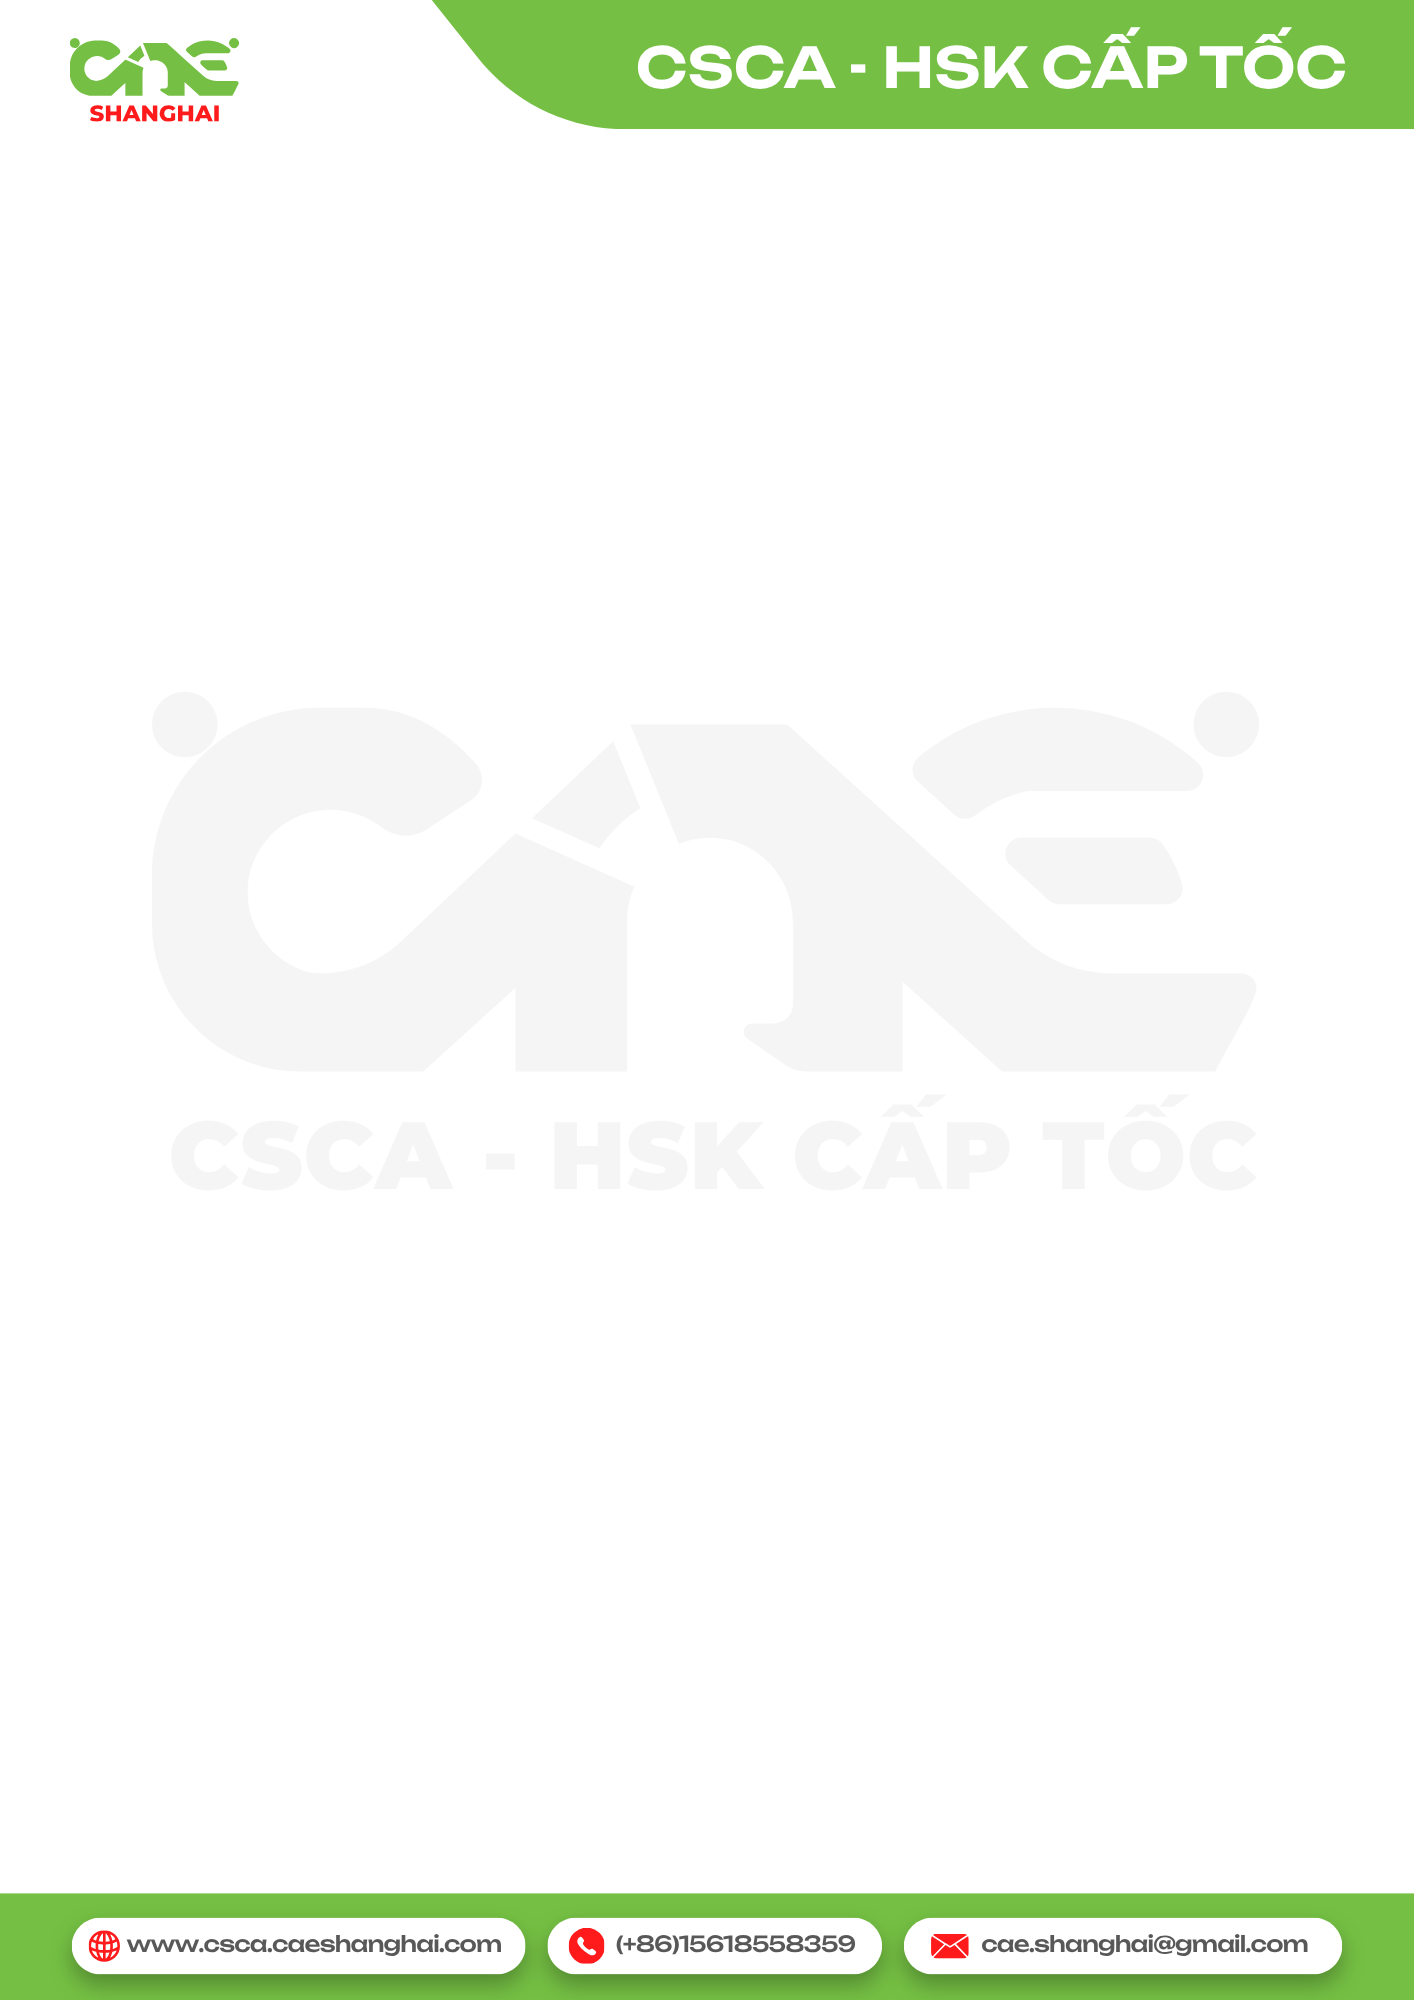
\includegraphics[width=\paperwidth,height=\paperheight]{images/letterhead.png}%
  }%
}

% ---------- ĐẦU / CHÂN TRANG ----------
% Letterhead đã có banner trên và dưới, nên bỏ dòng chạy để tránh chồng chữ.
% Số trang đặt trong vùng nội dung, sát trên banner dưới, lề phải.
\pagestyle{fancy}
\setlength{\headheight}{0pt}
\fancyhf{}
\renewcommand{\headrulewidth}{0pt}
\renewcommand{\footrulewidth}{0pt}
\fancyfoot[R]{\raisebox{0.9cm}{\small\color{cae_blue}\thepage}}

% ---------- MÔI TRƯỜNG NỘI DUNG ----------
% Trong tcolorbox, LaTeX đặt parindent = parskip = 0, nên các đoạn văn trong
% khung dính liền nhau. Đặt lại khoảng cách đoạn cho mọi khung.
\newcommand{\khoangcachdoan}{\setlength{\parskip}{0.5em}\setlength{\parindent}{0pt}}
\tcbset{before upper={\khoangcachdoan}}

\newtcolorbox{dinhnghia}[1][]{
  colback=box_bg, colframe=box_line, boxrule=0.6pt, arc=1pt,
  fonttitle=\bfseries, title={Định nghĩa #1}, breakable}
\newtcolorbox{dinhly}[1][]{
  colback=box_bg, colframe=cae_gold, boxrule=0.6pt, arc=1pt,
  fonttitle=\bfseries, title={Tính chất #1}, breakable}
\newtcolorbox{vidu}[1][]{
  colback=white, colframe=black!40, boxrule=0.4pt, arc=1pt,
  fonttitle=\bfseries, title={Ví dụ #1}, breakable}
\newtcolorbox{baitap}[1][]{
  colback=white, colframe=cae_blue!50, boxrule=0.4pt, arc=1pt,
  fonttitle=\bfseries, title={Câu #1}, breakable}

% Ô đáp án: viền xanh đậm hơn, dùng trong file đáp án
\newtcolorbox{dapan}[1][]{
  colback=box_bg, colframe=cae_blue, boxrule=0.6pt, arc=1pt,
  fonttitle=\bfseries, title={Câu #1}, breakable}

% ---------- TÊN CHỨNG MINH ----------
\renewcommand{\proofname}{\normalfont\bfseries Chứng minh}

% ---------- MÔN HỌC ----------
% Đổi được ở file .tex trước khi \input{cae-style} bằng \renewcommand{\monhoc}{...}
\providecommand{\monhoc}{Môn Toán}

% ---------- TRANG BÌA GỌN ----------
% #1 = loại tài liệu (TÀI LIỆU CHUẨN BỊ, TÀI LIỆU BUỔI HỌC, ...)
% #2 = số buổi
% #3 = tên buổi tiếng Việt
% #4 = tên buổi tiếng Hán
% #5 = module và tỉ trọng
\newcommand{\trangbia}[5]{%
  \begin{center}
    \vspace*{0.6cm}
    {\large\bfseries\color{cae_blue} CAE SHANGHAI}\\[0.15cm]
    {\footnotesize Tài liệu luyện thi CSCA · \monhoc}\\[0.5cm]
    {\color{cae_gold}\rule{0.55\linewidth}{0.8pt}}\\[0.35cm]
    {\small\bfseries\color{cae_blue!80!black} #1}\\[0.35cm]
    {\Large\bfseries\color{cae_blue} BUỔI #2 — #3}\\[0.2cm]
    {\large\color{cae_blue!85!black} \cjk{#4}}\\[0.25cm]
    \ifx\relax#5\relax\else{\small #5}\\[0.35cm]\fi
    {\color{cae_gold}\rule{0.55\linewidth}{0.8pt}}\\[0.3cm]
    {\footnotesize Biên soạn: Hoàng Dương, CAE Shanghai \quad·\quad \today}
  \end{center}
  \vspace{0.3cm}
}

% ---------- TRANG BÌA CHO ĐỀ KIỂM TRA ----------
% Khác \trangbia ở chỗ không có chữ "BUỔI N" — dùng cho đề thi, không phải bài giảng.
% #1 = loại tài liệu, #2 = tên kỳ thi (Việt), #3 = tên kỳ thi (Hán), #4 = thông số
\newcommand{\biade}[4]{%
  \begin{center}
    \vspace*{0.6cm}
    {\large\bfseries\color{cae_blue} CAE SHANGHAI}\\[0.15cm]
    {\footnotesize Tài liệu luyện thi CSCA · \monhoc}\\[0.5cm]
    {\color{cae_gold}\rule{0.55\linewidth}{0.8pt}}\\[0.35cm]
    {\small\bfseries\color{cae_blue!80!black} #1}\\[0.35cm]
    {\Large\bfseries\color{cae_blue} #2}\\[0.2cm]
    {\large\color{cae_blue!85!black} \cjk{#3}}\\[0.25cm]
    {\small #4}\\[0.35cm]
    {\color{cae_gold}\rule{0.55\linewidth}{0.8pt}}\\[0.3cm]
    {\footnotesize Biên soạn: Hoàng Dương, CAE Shanghai \quad·\quad \today}
  \end{center}
  \vspace{0.3cm}
}

% ---------- TIỆN ÍCH ----------
% Nhãn từ khóa in đậm ở đầu đoạn, dùng cho Từ vựng / Từ khóa nhận dạng / Chú ý
% Khoảng cách đoạn do khung tự đặt (xem \khoangcachdoan ở trên),
% ở đây chỉ cần tách đoạn và bỏ thụt đầu dòng.
\newcommand{\nhan}[1]{\par\noindent\textbf{#1.}\ \ignorespaces}

% Bảng gọn, không đánh số
\newcommand{\bang}[1]{%
  \begin{center}#1\end{center}}

% Đánh dấu ô trống cho học sinh điền
\newcommand{\chotrong}{\makebox[3.2cm]{\dotfill}}
 bằng \renewcommand{\monhoc}{...}
\providecommand{\monhoc}{Môn Toán}

% ---------- TRANG BÌA GỌN ----------
% #1 = loại tài liệu (TÀI LIỆU CHUẨN BỊ, TÀI LIỆU BUỔI HỌC, ...)
% #2 = số buổi
% #3 = tên buổi tiếng Việt
% #4 = tên buổi tiếng Hán
% #5 = module và tỉ trọng
\newcommand{\trangbia}[5]{%
  \begin{center}
    \vspace*{0.6cm}
    {\large\bfseries\color{cae_blue} CAE SHANGHAI}\\[0.15cm]
    {\footnotesize Tài liệu luyện thi CSCA · \monhoc}\\[0.5cm]
    {\color{cae_gold}\rule{0.55\linewidth}{0.8pt}}\\[0.35cm]
    {\small\bfseries\color{cae_blue!80!black} #1}\\[0.35cm]
    {\Large\bfseries\color{cae_blue} BUỔI #2 — #3}\\[0.2cm]
    {\large\color{cae_blue!85!black} \cjk{#4}}\\[0.25cm]
    \ifx\relax#5\relax\else{\small #5}\\[0.35cm]\fi
    {\color{cae_gold}\rule{0.55\linewidth}{0.8pt}}\\[0.3cm]
    {\footnotesize Biên soạn: Hoàng Dương, CAE Shanghai \quad·\quad \today}
  \end{center}
  \vspace{0.3cm}
}

% ---------- TRANG BÌA CHO ĐỀ KIỂM TRA ----------
% Khác \trangbia ở chỗ không có chữ "BUỔI N" — dùng cho đề thi, không phải bài giảng.
% #1 = loại tài liệu, #2 = tên kỳ thi (Việt), #3 = tên kỳ thi (Hán), #4 = thông số
\newcommand{\biade}[4]{%
  \begin{center}
    \vspace*{0.6cm}
    {\large\bfseries\color{cae_blue} CAE SHANGHAI}\\[0.15cm]
    {\footnotesize Tài liệu luyện thi CSCA · \monhoc}\\[0.5cm]
    {\color{cae_gold}\rule{0.55\linewidth}{0.8pt}}\\[0.35cm]
    {\small\bfseries\color{cae_blue!80!black} #1}\\[0.35cm]
    {\Large\bfseries\color{cae_blue} #2}\\[0.2cm]
    {\large\color{cae_blue!85!black} \cjk{#3}}\\[0.25cm]
    {\small #4}\\[0.35cm]
    {\color{cae_gold}\rule{0.55\linewidth}{0.8pt}}\\[0.3cm]
    {\footnotesize Biên soạn: Hoàng Dương, CAE Shanghai \quad·\quad \today}
  \end{center}
  \vspace{0.3cm}
}

% ---------- TIỆN ÍCH ----------
% Nhãn từ khóa in đậm ở đầu đoạn, dùng cho Từ vựng / Từ khóa nhận dạng / Chú ý
% Khoảng cách đoạn do khung tự đặt (xem \khoangcachdoan ở trên),
% ở đây chỉ cần tách đoạn và bỏ thụt đầu dòng.
\newcommand{\nhan}[1]{\par\noindent\textbf{#1.}\ \ignorespaces}

% Bảng gọn, không đánh số
\newcommand{\bang}[1]{%
  \begin{center}#1\end{center}}

% Đánh dấu ô trống cho học sinh điền
\newcommand{\chotrong}{\makebox[3.2cm]{\dotfill}}
 bằng \renewcommand{\monhoc}{...}
\providecommand{\monhoc}{Môn Toán}

% ---------- TRANG BÌA GỌN ----------
% #1 = loại tài liệu (TÀI LIỆU CHUẨN BỊ, TÀI LIỆU BUỔI HỌC, ...)
% #2 = số buổi
% #3 = tên buổi tiếng Việt
% #4 = tên buổi tiếng Hán
% #5 = module và tỉ trọng
\newcommand{\trangbia}[5]{%
  \begin{center}
    \vspace*{0.6cm}
    {\large\bfseries\color{cae_blue} CAE SHANGHAI}\\[0.15cm]
    {\footnotesize Tài liệu luyện thi CSCA · \monhoc}\\[0.5cm]
    {\color{cae_gold}\rule{0.55\linewidth}{0.8pt}}\\[0.35cm]
    {\small\bfseries\color{cae_blue!80!black} #1}\\[0.35cm]
    {\Large\bfseries\color{cae_blue} BUỔI #2 — #3}\\[0.2cm]
    {\large\color{cae_blue!85!black} \cjk{#4}}\\[0.25cm]
    \ifx\relax#5\relax\else{\small #5}\\[0.35cm]\fi
    {\color{cae_gold}\rule{0.55\linewidth}{0.8pt}}\\[0.3cm]
    {\footnotesize Biên soạn: Hoàng Dương, CAE Shanghai \quad·\quad \today}
  \end{center}
  \vspace{0.3cm}
}

% ---------- TRANG BÌA CHO ĐỀ KIỂM TRA ----------
% Khác \trangbia ở chỗ không có chữ "BUỔI N" — dùng cho đề thi, không phải bài giảng.
% #1 = loại tài liệu, #2 = tên kỳ thi (Việt), #3 = tên kỳ thi (Hán), #4 = thông số
\newcommand{\biade}[4]{%
  \begin{center}
    \vspace*{0.6cm}
    {\large\bfseries\color{cae_blue} CAE SHANGHAI}\\[0.15cm]
    {\footnotesize Tài liệu luyện thi CSCA · \monhoc}\\[0.5cm]
    {\color{cae_gold}\rule{0.55\linewidth}{0.8pt}}\\[0.35cm]
    {\small\bfseries\color{cae_blue!80!black} #1}\\[0.35cm]
    {\Large\bfseries\color{cae_blue} #2}\\[0.2cm]
    {\large\color{cae_blue!85!black} \cjk{#3}}\\[0.25cm]
    {\small #4}\\[0.35cm]
    {\color{cae_gold}\rule{0.55\linewidth}{0.8pt}}\\[0.3cm]
    {\footnotesize Biên soạn: Hoàng Dương, CAE Shanghai \quad·\quad \today}
  \end{center}
  \vspace{0.3cm}
}

% ---------- TIỆN ÍCH ----------
% Nhãn từ khóa in đậm ở đầu đoạn, dùng cho Từ vựng / Từ khóa nhận dạng / Chú ý
% Khoảng cách đoạn do khung tự đặt (xem \khoangcachdoan ở trên),
% ở đây chỉ cần tách đoạn và bỏ thụt đầu dòng.
\newcommand{\nhan}[1]{\par\noindent\textbf{#1.}\ \ignorespaces}

% Bảng gọn, không đánh số
\newcommand{\bang}[1]{%
  \begin{center}#1\end{center}}

% Đánh dấu ô trống cho học sinh điền
\newcommand{\chotrong}{\makebox[3.2cm]{\dotfill}}


\begin{document}

\trangbia{TÀI LIỆU BUỔI HỌC}{4}{LƯỢNG GIÁC: GIÁ TRỊ VÀ CÔNG THỨC BIẾN ĐỔI}{三角函数·恒等变换}{Module M2 \quad·\quad Tỉ trọng đề thi $\sim$20\% (cả chuyên đề Lượng giác) \quad·\quad khoảng 8–11 câu}

\section{TỪ KHÓA NHẬN DẠNG ĐỀ}

Đọc được từ khóa là xác định được dạng bài mà không cần dịch cả đề. Bảng dưới đây gom những từ khóa quyết định của chuyên đề này.

\bang{
\begin{tabularx}{\linewidth}{@{\hspace{6pt}}llX@{\hspace{6pt}}}
\toprule
\textbf{Từ khóa} & \textbf{Nghĩa} & \textbf{Dạng bài tương ứng} \\
\midrule
求值 & tính giá trị & Thay số vào công thức lượng giác \\
化简 & rút gọn & Biến đổi biểu thức về dạng đơn giản \\
恒等式 & đẳng thức & Chứng minh hai vế bằng nhau \\
象限角 & góc phần tư & Xác định dấu của giá trị lượng giác \\
终边 & tia cuối của góc & Cho điểm trên tia cuối, tính tỉ số \\
正弦 / 余弦 / 正切 & sin / cos / tan & Chọn đúng hàm theo đề hỏi \\
二倍角 & góc nhân đôi & Dùng $\sin 2\alpha$, $\cos 2\alpha$, $\tan 2\alpha$ \\
两角和 / 两角差 & tổng / hiệu hai góc & Dùng công thức cộng \\
半角 & góc chia đôi & Dùng công thức hạ bậc \\
最大值 / 最小值 & giá trị lớn nhất / nhỏ nhất & Đưa về $R\sin(x+\varphi)$ \\
最小正周期 & chu kỳ dương nhỏ nhất & Đọc hệ số của $x$ trong hàm sin, cos \\
奇函数 / 偶函数 & hàm lẻ / hàm chẵn & Xét $f(-x)$ với hàm lượng giác \\
\bottomrule
\end{tabularx}}

\nhan{Chú ý} Bốn từ 正弦, 余弦, 正切, 余切 ứng với bốn hàm sin, cos, tan, cot. Đề rất hay hỏi 正切 (tan) trong khi biểu thức cho sẵn dưới dạng sin và cos. Nhận ra điều này là biết ngay phải chia cả tử và mẫu cho $\cos\alpha$.

\section{KIẾN THỨC TRỌNG TÂM}

\subsection{Cung, góc và giá trị lượng giác}

\begin{dinhnghia}[{1 — Góc lượng giác và tia cuối}]
Trong mặt phẳng tọa độ, góc $\alpha$ có cạnh đầu là chiều dương trục $Ox$ và cạnh cuối là tia $OM$. Lấy $M(x, y)$ khác gốc, đặt $r = \sqrt{x^2 + y^2} > 0$. Khi đó:

$$\sin\alpha = \frac{y}{r}, \qquad \cos\alpha = \frac{x}{r}, \qquad \tan\alpha = \frac{y}{x}\ (x \neq 0), \qquad \cot\alpha = \frac{x}{y}\ (y \neq 0)$$
\end{dinhnghia}
\begin{dinhnghia}[{2 — Radian}]
Góc có độ dài cung bằng bán kính gọi là góc $1$ radian. Công thức liên hệ:

$$\pi \ \text{rad} = 180^\circ, \qquad l = |\alpha| r$$

trong đó $l$ là độ dài cung và $r$ là bán kính.
\end{dinhnghia}
\begin{dinhly}[{1 — Dấu của giá trị lượng giác theo phần tư}]
\bang{
\begin{tabularx}{\linewidth}{@{\hspace{6pt}}Xccc@{\hspace{6pt}}}
\toprule
\textbf{Phần tư} & \textbf{$\sin\alpha$} & \textbf{$\cos\alpha$} & \textbf{$\tan\alpha$} \\
\midrule
I & $+$ & $+$ & $+$ \\
II & $+$ & $-$ & $-$ \\
III & $-$ & $-$ & $+$ \\
IV & $-$ & $+$ & $-$ \\
\bottomrule
\end{tabularx}}

\nhan{Chú ý} Quy tắc nhớ: $\sin$ dương ở hai phần tư trên (I, II), $\cos$ dương ở hai phần tư bên phải (I, IV), $\tan$ dương ở hai phần tư chéo (I, III). Đề cho 象限角 là đề đang hỏi dấu, không phải hỏi độ lớn.
\end{dinhly}
\begin{dinhly}[{2 — Giá trị lượng giác của cung đặc biệt}]
\bang{
\begin{tabular*}{\linewidth}{@{\extracolsep{\fill}\hspace{6pt}}lccccc@{\hspace{6pt}}}
\toprule
\textbf{$\alpha$} & \textbf{$0$} & \textbf{$\dfrac{\pi}{6}$} & \textbf{$\dfrac{\pi}{4}$} & \textbf{$\dfrac{\pi}{3}$} & \textbf{$\dfrac{\pi}{2}$} \\
\midrule
$\sin\alpha$ & $0$ & $\dfrac{1}{2}$ & $\dfrac{\sqrt{2}}{2}$ & $\dfrac{\sqrt{3}}{2}$ & $1$ \\
$\cos\alpha$ & $1$ & $\dfrac{\sqrt{3}}{2}$ & $\dfrac{\sqrt{2}}{2}$ & $\dfrac{1}{2}$ & $0$ \\
$\tan\alpha$ & $0$ & $\dfrac{\sqrt{3}}{3}$ & $1$ & $\sqrt{3}$ & không xác định \\
\bottomrule
\end{tabular*}}
\end{dinhly}
\subsection{Quan hệ cơ bản và cung liên kết}

\begin{dinhly}[{3 — Hệ thức lượng giác cơ bản}]
$$\sin^2\alpha + \cos^2\alpha = 1, \qquad \tan\alpha = \frac{\sin\alpha}{\cos\alpha}, \qquad \tan\alpha \cdot \cot\alpha = 1$$

\textbf{Hệ quả.} $1 + \tan^2\alpha = \dfrac{1}{\cos^2\alpha}$.

\nhan{Chú ý} Từ $\sin^2\alpha + \cos^2\alpha = 1$ suy ra $|\sin\alpha| \le 1$ và $|\cos\alpha| \le 1$. Đây là công cụ loại trừ đáp án nhanh: giá trị nào có trị tuyệt đối lớn hơn $1$ thì không thể là $\sin\alpha$ hay $\cos\alpha$.
\end{dinhly}
\begin{dinhly}[{4 — Cung đối, cung bù, cung phụ}]
Với mọi $\alpha$:

$$\sin(-\alpha) = -\sin\alpha, \qquad \cos(-\alpha) = \cos\alpha, \qquad \tan(-\alpha) = -\tan\alpha$$

$$\sin(\pi - \alpha) = \sin\alpha, \qquad \cos(\pi - \alpha) = -\cos\alpha, \qquad \tan(\pi - \alpha) = -\tan\alpha$$

$$\sin\!\left(\frac{\pi}{2} - \alpha\right) = \cos\alpha, \qquad \cos\!\left(\frac{\pi}{2} - \alpha\right) = \sin\alpha$$

\nhan{Cách nhanh} Cung phụ đổi tên hàm (sin thành cos), cung bù và cung đối giữ nguyên tên hàm. Dấu lấy theo phần tư của góc kết quả.
\end{dinhly}
\begin{dinhly}[{5 — Công thức cộng}]
$$\sin(\alpha \pm \beta) = \sin\alpha\cos\beta \pm \cos\alpha\sin\beta$$

$$\cos(\alpha \pm \beta) = \cos\alpha\cos\beta \mp \sin\alpha\sin\beta$$

$$\tan(\alpha \pm \beta) = \frac{\tan\alpha \pm \tan\beta}{1 \mp \tan\alpha\tan\beta}$$

\nhan{Chú ý} Với công thức cos, dấu ở hai vế \textbf{ngược nhau}: $\cos(\alpha + \beta)$ thì giữa hai tích là dấu trừ. Đây là chỗ sai phổ biến nhất khi học thuộc công thức cộng.
\end{dinhly}
\subsection{Công thức nhân đôi và hạ bậc}

\begin{dinhly}[{6 — Công thức nhân đôi}]
$$\sin 2\alpha = 2\sin\alpha\cos\alpha$$

$$\cos 2\alpha = \cos^2\alpha - \sin^2\alpha = 2\cos^2\alpha - 1 = 1 - 2\sin^2\alpha$$

$$\tan 2\alpha = \frac{2\tan\alpha}{1 - \tan^2\alpha}$$

\nhan{Chú ý} $\cos 2\alpha$ có \textbf{ba dạng} tương đương. Chọn dạng nào là tùy dữ kiện đề cho: cho $\sin\alpha$ thì dùng $1 - 2\sin^2\alpha$, cho $\cos\alpha$ thì dùng $2\cos^2\alpha - 1$.
\end{dinhly}
\begin{dinhly}[{7 — Công thức hạ bậc}]
$$\sin^2\alpha = \frac{1 - \cos 2\alpha}{2}, \qquad \cos^2\alpha = \frac{1 + \cos 2\alpha}{2}$$

\textbf{Hệ quả.} $\tan\dfrac{\alpha}{2} = \dfrac{\sin\alpha}{1 + \cos\alpha}$.

\nhan{Cách nhanh} Biểu thức có bậc hai của sin hoặc cos thì nghĩ ngay đến hạ bậc. Đây là bước đầu tiên của hầu hết bài rút gọn lượng giác.
\end{dinhly}
\subsection{Biến đổi tổng thành tích và tích thành tổng}

\begin{dinhly}[{8 — Công thức biến đổi tích thành tổng}]
$$\sin\alpha\cos\beta = \frac{1}{2}\big[\sin(\alpha+\beta) + \sin(\alpha-\beta)\big]$$

$$\cos\alpha\cos\beta = \frac{1}{2}\big[\cos(\alpha+\beta) + \cos(\alpha-\beta)\big]$$

$$\sin\alpha\sin\beta = -\frac{1}{2}\big[\cos(\alpha+\beta) - \cos(\alpha-\beta)\big]$$
\end{dinhly}
\begin{dinhly}[{9 — Công thức biến đổi tổng thành tích}]
$$\sin x + \sin y = 2\sin\frac{x+y}{2}\cos\frac{x-y}{2}, \qquad \sin x - \sin y = 2\cos\frac{x+y}{2}\sin\frac{x-y}{2}$$

$$\cos x + \cos y = 2\cos\frac{x+y}{2}\cos\frac{x-y}{2}, \qquad \cos x - \cos y = -2\sin\frac{x+y}{2}\sin\frac{x-y}{2}$$
\end{dinhly}
\begin{dinhly}[{10 — Công thức gộp bậc nhất sin và cos}]
Với $a, b$ không đồng thời bằng $0$:

$$a\sin x + b\cos x = \sqrt{a^2+b^2}\,\sin(x + \varphi)$$

trong đó $\varphi$ xác định bởi $\cos\varphi = \dfrac{a}{\sqrt{a^2+b^2}}$, $\sin\varphi = \dfrac{b}{\sqrt{a^2+b^2}}$.

\textbf{Hệ quả.} $-\sqrt{a^2+b^2} \le a\sin x + b\cos x \le \sqrt{a^2+b^2}$.

\nhan{Cách nhanh} Đây là công thức cho đáp án trong vài giây. Biểu thức $a\sin x + b\cos x$ có giá trị lớn nhất là $\sqrt{a^2+b^2}$ và nhỏ nhất là $-\sqrt{a^2+b^2}$, không cần biến đổi.

\end{dinhly}
\section{CÁC DẠNG BÀI}

\subsection{Dạng 1 — Tính giá trị lượng giác khi biết một giá trị và phần tư}

\nhan{Cách nhận dạng} Đề cho một giá trị lượng giác (thường là $\sin\alpha$ hoặc $\tan\alpha$) kèm từ khóa 象限角, yêu cầu tính giá trị còn lại.

\nhan{Cách làm} Dùng $\sin^2\alpha + \cos^2\alpha = 1$ để tìm trị tuyệt đối của giá trị cần tính, sau đó dùng phần tư để chọn dấu.

\begin{vidu}[{1}]
Cho $\sin\alpha = -\dfrac{1}{2}$ và $\alpha$ là góc phần tư thứ ba. Tính $\cos\alpha$.

Từ $\sin^2\alpha + \cos^2\alpha = 1$:

$$\cos^2\alpha = 1 - \left(-\frac{1}{2}\right)^2 = 1 - \frac{1}{4} = \frac{3}{4} \implies |\cos\alpha| = \frac{\sqrt{3}}{2}$$

Góc phần tư thứ ba có $\cos\alpha < 0$, vậy $\cos\alpha = -\dfrac{\sqrt{3}}{2}$.

\end{vidu}
\subsection{Dạng 2 — Rút gọn biểu thức lượng giác}

\nhan{Cách nhận dạng} Đề có từ khóa 化简, biểu thức chứa nhiều hàm lượng giác lẫn lộn, thường có phân thức.

\nhan{Cách làm} Quy về cùng một hàm (thường là sin và cos), dùng $\sin^2\alpha + \cos^2\alpha = 1$ và hạ bậc để triệt tiêu nhân tử chung.

\begin{vidu}[{2}]
Rút gọn $\dfrac{\sin^2 x}{1 - \cos x}$ với $\cos x \neq 1$.

Thay $\sin^2 x = 1 - \cos^2 x = (1-\cos x)(1+\cos x)$:

$$\frac{\sin^2 x}{1 - \cos x} = \frac{(1-\cos x)(1+\cos x)}{1 - \cos x} = 1 + \cos x$$

\end{vidu}
\subsection{Dạng 3 — Biểu thức đối xứng của sin và cos}

\nhan{Cách nhận dạng} Đề cho $\tan\alpha$ (hoặc $\sin\alpha \pm \cos\alpha$) và yêu cầu tính một phân thức bậc nhất hai ẩn $\sin\alpha$, $\cos\alpha$.

\nhan{Cách làm} Chia cả tử và mẫu cho $\cos\alpha$ để đưa toàn bộ về $\tan\alpha$. Với phân thức đối xứng bậc hai, chia cho $\cos^2\alpha$.

\begin{vidu}[{3}]
Cho $\tan\alpha = 2$. Tính $\dfrac{\sin\alpha - \cos\alpha}{\sin\alpha + \cos\alpha}$.

Vì $\tan\alpha = 2$ nên $\cos\alpha \neq 0$. Chia cả tử và mẫu cho $\cos\alpha$:

$$\frac{\sin\alpha - \cos\alpha}{\sin\alpha + \cos\alpha} = \frac{\tan\alpha - 1}{\tan\alpha + 1} = \frac{2 - 1}{2 + 1} = \frac{1}{3}$$

\nhan{Cách nhanh} Không cần tìm $\sin\alpha$ và $\cos\alpha$ riêng lẻ. Chỉ cần một phép chia là ra đáp án.

\end{vidu}
\subsection{Dạng 4 — Tính giá trị bằng công thức cộng và nhân đôi}

\nhan{Cách nhận dạng} Đề cho một giá trị lượng giác của $\alpha$ và hỏi giá trị của $\alpha + \beta$ với $\beta$ là góc đặc biệt ($\dfrac{\pi}{4}$, $\dfrac{\pi}{3}$, $\dfrac{\pi}{6}$), hoặc hỏi giá trị của $2\alpha$.

\nhan{Cách làm} Nhận ra $\beta$ là góc đặc biệt, thay trực tiếp vào công thức cộng. Với góc nhân đôi, dùng Tính chất 6.

\begin{vidu}[{4}]
Cho $\tan\alpha = 2$. Tính $\tan\!\left(\alpha + \dfrac{\pi}{4}\right)$.

Áp dụng công thức cộng với $\tan\dfrac{\pi}{4} = 1$:

$$\tan\!\left(\alpha + \frac{\pi}{4}\right) = \frac{\tan\alpha + \tan\frac{\pi}{4}}{1 - \tan\alpha\tan\frac{\pi}{4}} = \frac{2 + 1}{1 - 2 \cdot 1} = \frac{3}{-1} = -3$$

\end{vidu}
\subsection{Dạng 5 — Chứng minh đẳng thức lượng giác}

\nhan{Cách nhận dạng} Đề có từ khóa 恒等式 hoặc yêu cầu 证明 (chứng minh), hai vế là hai biểu thức lượng giác.

\nhan{Cách làm} Biến đổi vế phức tạp hơn về vế đơn giản hơn. Với đẳng thức chứa bậc hai, hạ bậc trước. Với đẳng thức chứa tổng của sin và cos, dùng công thức biến đổi tổng thành tích.

\begin{vidu}[{5}]
Chứng minh $\sin 2\alpha = 2\sin\alpha\cos\alpha$ bằng công thức cộng.

Viết $2\alpha = \alpha + \alpha$ rồi áp dụng công thức cộng:

$$\sin 2\alpha = \sin(\alpha + \alpha) = \sin\alpha\cos\alpha + \cos\alpha\sin\alpha = 2\sin\alpha\cos\alpha$$

\end{vidu}
\subsection{Dạng 6 — Giá trị lớn nhất, nhỏ nhất của biểu thức lượng giác}

\nhan{Cách nhận dạng} Đề có từ khóa 最大值 hoặc 最小值, biểu thức là bậc nhất theo $\sin x$ và $\cos x$, hoặc bậc hai của một hàm lượng giác.

\nhan{Cách làm} Với $a\sin x + b\cos x$, dùng Tính chất 10 để kết luận ngay giá trị lớn nhất là $\sqrt{a^2+b^2}$. Với $\sin^2 x$ hoặc $\cos^2 x$, hạ bậc rồi dùng $|\cos 2x| \le 1$.

\begin{vidu}[{6}]
Tìm giá trị lớn nhất của $y = \sin x + \cos x$.

Áp dụng Tính chất 10 với $a = b = 1$:

$$y = \sqrt{1^2 + 1^2}\,\sin\!\left(x + \frac{\pi}{4}\right) = \sqrt{2}\sin\!\left(x + \frac{\pi}{4}\right)$$

Vì $|\sin| \le 1$ nên giá trị lớn nhất của $y$ là $\sqrt{2}$, đạt được khi $x = \dfrac{\pi}{4}$.

\nhan{Cách nhanh} Nhớ công thức $\max(a\sin x + b\cos x) = \sqrt{a^2+b^2}$ để trả lời trong $5$ giây.

\end{vidu}
\subsection{Dạng 7 — Chu kỳ và tính chẵn lẻ của hàm số lượng giác}

\nhan{Cách nhận dạng} Đề có từ khóa 最小正周期 (chu kỳ dương nhỏ nhất) hoặc 奇函数 / 偶函数, hàm số chứa sin hoặc cos.

\nhan{Cách làm} Với $y = \sin(\omega x + \varphi)$ hoặc $y = \cos(\omega x + \varphi)$, chu kỳ là $T = \dfrac{2\pi}{|\omega|}$. Với tính chẵn lẻ, thay $-x$ và so sánh với $f(x)$: nếu $f(-x) = f(x)$ thì hàm chẵn, nếu $f(-x) = -f(x)$ thì hàm lẻ.

\begin{vidu}[{7}]
Tìm chu kỳ của $f(x) = \sin\!\left(4x - \dfrac{\pi}{3}\right)$.

Hệ số của $x$ là $\omega = 4$, vậy:

$$T = \frac{2\pi}{|4|} = \frac{\pi}{2}$$

\nhan{Chú ý} Hệ số tự do $\varphi = -\dfrac{\pi}{3}$ \textbf{không ảnh hưởng} đến chu kỳ. Chỉ đọc $\omega$ là đủ.

\end{vidu}
\section{PHỤ LỤC — BỐI CẢNH KỲ THI}

\subsection{Cấu trúc đề thi CSCA môn Toán}

\bang{
\begin{tabularx}{\linewidth}{@{\hspace{6pt}}lX@{\hspace{6pt}}}
\toprule
\textbf{Đặc điểm} & \textbf{Thông số} \\
\midrule
Số câu & 48 câu trắc nghiệm \\
Thời gian & 60 phút \\
Thang điểm & 100 điểm \\
Ngôn ngữ & Tiếng Trung hoặc tiếng Anh (thí sinh chọn) \\
Máy tính & Không được dùng \\
\bottomrule
\end{tabularx}}

Thời gian trung bình mỗi câu là \textbf{1 phút 15 giây}. Mục tiêu của khóa học không phải giải được bài khó, mà là \textbf{nhận ra dạng bài trong vài giây và chọn đúng đáp án trong khoảng 40 giây}.

\subsection{Trọng số các nhóm nội dung}

\bang{
\begin{tabularx}{\linewidth}{@{\hspace{6pt}}Xcc@{\hspace{6pt}}}
\toprule
\textbf{Nhóm nội dung} & \textbf{Số câu} & \textbf{Tỉ trọng} \\
\midrule
\textbf{Lượng giác} & \textbf{8–11} & \textbf{~20\%} \\
Hình học giải tích & 8–10 & ~19\% \\
Dãy số & 5–8 & ~13\% \\
Hàm số & 5–7 & ~13\% \\
Tập hợp \& bất đẳng thức & 4–6 & ~10\% \\
Mũ \& logarit & 3–5 & ~8\% \\
Vector \& số phức & 2–4 & ~6\% \\
Xác suất \& thống kê & 1–2 & ~3\% \\
\bottomrule
\end{tabularx}}

Lượng giác là nhóm nội dung \textbf{lớn nhất} trong đề thi, chiếm khoảng 20\%. Buổi này xử lý phần giá trị và công thức biến đổi, buổi 5 xử lý hàm số và phương trình lượng giác.

\subsection{Bảng giá trị lượng giác cần thuộc}

\bang{
\begin{tabular*}{\linewidth}{@{\extracolsep{\fill}\hspace{6pt}}lccccccc@{\hspace{6pt}}}
\toprule
\textbf{$\alpha$} & \textbf{$0$} & \textbf{$\dfrac{\pi}{6}$} & \textbf{$\dfrac{\pi}{4}$} & \textbf{$\dfrac{\pi}{3}$} & \textbf{$\dfrac{\pi}{2}$} & \textbf{$\dfrac{2\pi}{3}$} & \textbf{$\pi$} \\
\midrule
$\sin\alpha$ & $0$ & $\dfrac{1}{2}$ & $\dfrac{\sqrt{2}}{2}$ & $\dfrac{\sqrt{3}}{2}$ & $1$ & $\dfrac{\sqrt{3}}{2}$ & $0$ \\
$\cos\alpha$ & $1$ & $\dfrac{\sqrt{3}}{2}$ & $\dfrac{\sqrt{2}}{2}$ & $\dfrac{1}{2}$ & $0$ & $-\dfrac{1}{2}$ & $-1$ \\
$\tan\alpha$ & $0$ & $\dfrac{\sqrt{3}}{3}$ & $1$ & $\sqrt{3}$ & không xác định & $-\sqrt{3}$ & $0$ \\
\bottomrule
\end{tabular*}}
\vspace{0.8cm}
\begin{center}
{\footnotesize\color{cae_blue} Tài liệu nội bộ, CAE SHANGHAI}
\end{center}

\end{document}
